\chapter{Analyse von Deadlock-Go und Vergleich mit 
    go-deadlock (sasha-s)}
Im Folgenden soll der in Kap. \ref{Kap::Implementaion} beschriebene und in 
\cite{implementation} implementierte Detektor \glqq Deadlock-Go\grqq\ analysiert 
und mit dem in 
\ref{Chap::Review:go-deadlock} betrachteten Detektor \glqq go-deadlock\grqq\ verglichen
werden. Um Verwechslungen zwischen den beiden relativ ähnlichen Namen zu vermeiden,
wird dieser im folgenden nach dem Besitzer des Git-Hub Repositories als sasha-s
bezeichnet.\\
Für den Vergleich werden verschiedene Beispiel-Programme betrachtet, die in 
\cite{examples} implementiert sind. Diese bestehen zum einen aus verschiedenen 
Standartsituationen, zum anderen auf Programmen, die aus tatsächlichen
Programmen übernommen wurden. Diese werden aus Gobench \cite{gobench}, einer 
Benchmark Suite für Parallelitätsfehler in Go ausgewählt.
\section{Funktionale Analyse}
Man analysiere die Programme zuerst funktional, d.h. man überprüfe, ob sie zu den 
gewünschten Ergebnissen führen.\\
Man betrachte zuerst die Standardsituationen. In der folgenden Tabelle 
\ref{Tab::Analyse:Functional.Standart} sind die 
betrachteten Situation beschrieben. Dazu wird für jede Situation eine kurze 
Beschreibung angegeben und dann überprüft, ob die beiden Detektoren in der Lage 
sind diese korrekt zu klassifizieren, d.h. ein Warnung über einen Deadlock auszugeben,
wenn ein solcher vorliegt, und keine Warnung zu geben, wenn kein Deadlock auftreten
kann.\\\\
Ein potenzielles Deadlock, welches 
durch das zyklische Locking von zwei Deadlocks auftritt kann durch beide Tools
erkannt werden (1.1). Ebenso erkenne beide, dass kein Deadlock vorliegt, wenn das 
Locking von mehreren Locks nicht zyklisch verläuft (1.2).
Sobald diese Zyklen allerdings eine Länge von 3 oder mehr 
erreichen, werden diese durch sasha-s nicht mehr erkannt, da dieser 
Detektor nur nach Zyklen der Länge zwei sucht (2). Deadlock-Go 
hingegen ist in der Lage auch diese potenziellen Deadlocks zu erkennen.\\
Auch bei Deadlocks, in denen zwar zyklisches Locking auftritt, welche aber 
auf Grund von Gate-Locks nicht zu einem tatsächlich Deadlock führen können,
schneidet Deadlock-Go besser ab (3). Da dieser mit Lock-Bäumen und nicht mit einem
Lock-Graphen implementiert ist, wird in diesem Fall kein potenzielles Deadlock 
ausgegeben. sasha-s hingegen erkennt nicht, dass solch ein Deadlock nicht 
auftreten kann und gibt somit eine false-positive Mitteilung über ein potenzielles 
Deadlock aus.\\ 
sasha-s ist standardmäßig dazu in  der Lage doppeltes Locking zu erkennen.
Bei Deadlock-Go hängt die Erkennung solcher Deadlocks von den Optionen ab.
Ist die Erkennung von doppeltem Locking nicht deaktiviert, ist Deadlock-Go also auch in 
der Lage solche Deadlocks durch doppeltes Locking zu erkennen (5). \\ 
Bei verschachtelten Routinen ist 
keines der Tools in der Lage das potenzielle Deadlock zu erkennen (4).\\
Für tatsächlich auftretende Deadlocks, welche durch zyklisches Locking auftreten 
sind beide Detektoren in der Lage, solche Situationen zu erkennen (6).\\\\
Für sasha-s sind keine Try-Lock-Operationen implementiert. Aus diesem Grund 
können potenzielle Deadlocks, die solche Try-Lock Operationen besitzen nicht 
wirklich erkannt werden.\\Deadlock-Go besitzt eine Implementierung von Try-Lock-
Operationen. Doppeltes Locking kann für Try-Lock erkannt werden, sowohl wenn 
es auch bei ein Try-Lock zu doppeltem Locking kommt (7.1), als auch wenn es
durch die Try-Lock-Operation doppeltes Locking verhindert wird (7.2). Deadlock-Go
ist nicht in der Lage Deadlocks zu erkennen, wenn dieses durch zyklisches Locking 
auftritt, wobei der Zyklus ein Try-Lock enthält. Es wird kein potenzieller
Deadlock erkannt, unabhängig davon, ob der Zyklus mit dem Try-Lock zu einem  
Deadlock führen kann oder nicht (8).


\begin{table}[H]
\centering
\begin{tabular}{|l|l|l|l|}
    \hline
    \textbf{ID} & \textbf{Typ} & \textbf{Deadlock-Go} & \textbf{sasha-s} \\ \hline
    1.1 & potenzielles Deadlock durch zyklisches Locking von zwei Locks & Ja & Ja \\ \hline
    1.2 & Kein potenzielles Deadlock, da die Locks nicht zyklisch sind & Ja & Ja \\ \hline
    2 & potenzielles Deadlock durch zyklisches Locking von drei Locks & Ja & Nein \\ \hline
    3 & \makecell[l]{Zyklisches Locking welches aber durch Gate-Locks nicht\\zu einem Deadlock führen kann} & Ja & Nein \\ \hline
    4 & \makecell[l]{potenzielles Deadlock, welches durch Verschachtlung mehrerer\\Routinen (fork/join) verschleiert wird} & Nein & Nein \\ \hline
    5 & Deadlock durch doppeltes Locken & Ja & Ja \\ \hline
    6.1 & \makecell[l]{Tatsächliches Deadlock durch zyklisches Locking von Locks\\in zwei Routinen} & Ja & Ja \\ \hline
    6.2 & \makecell[l]{Tatsächliches Deadlock durch zyklisches Locking von Locks\\in drei Routinen} & Ja & Ja \\ \hline
    7.1 & Doppeltes Locking mit TryLock (TryLock $\to$ Lock) & Ja & Nein$^*$ \\ \hline
    7.2 & Kein doppeltes Locking mit TryLock (Lock $\to$ TryLock) & Ja & Nein$^*$\\ \hline
    8.1 & Deadlock durch zyklisches Locking mit TryLock & Nein &Nein$^*$ \\ \hline
    8.2 & \makecell[l]{Zyklisches Locking, welches durch TryLock nicht zu\\einem Deadlock führt} & Ja &Nein$^*$ \\ \hline   
    9.1 & \makecell[l]{potenzielles Deadlock mit RW-Lock in zwei Routinen\\(R1: x.RLock $\to$ y.Lock, R2: y.Lock $\to$ x.Lock)} & Ja & Ja \\ \hline
    9.2 & \makecell[l]{potenzielles Deadlock mit RW-Lock in zwei Routinen\\(R1: x.RLock $\to$ y.Lock, R2: y.RLock $\to$ x.Lock)} & Ja & Ja \\ \hline
    9.3 & \makecell[l]{Kein potenzielles Deadlock mit RW-Lock in zwei Routinen\\(R1: x.RLock $\to$ y.RLock, R2: y.RLock $\to$ x.RLock)} & Ja & Nein \\ \hline
    9.4 & \makecell[l]{Kein potenzielles Deadlock mit RW-Lock in zwei Routinen\\(R1: x.Lock $\to$ y.RLock, R2: y.RLock $\to$ x.Lock)} & Ja & Nein \\ \hline
    9.5 & \makecell[l]{Kein potenzielles Deadlock mit RW-Lock in zwei Routinen\\(R1: x.RLock $\to$ y.Lock, R2: y.RLock $\to$ x.RLock)} & Ja & Nein \\ \hline
    9.6 & \makecell[l]{Kein potenzielles Deadlock mit RW-Lock in zwei Routinen\\(R1: x.Lock $\to$ y.RLock, R2: y.RLock $\to$ x.RLock)} & Nein & Nein \\ \hline
    10.1 & \makecell[l]{Kein potenzielles Deadlock, wegen Lock von RW-Locks\\als Gate-Locks.} & Ja & Nein \\ \hline
    10.2 & \makecell[l]{potenzielles Deadlock, da R-Lock von Deadlock nicht als\\Gate-Lock funktioniert.} & Ja & Ja \\ \hline
    11.1 & \makecell[l]{Doppeltes Locking von RW-Locks, welches zu Deadlock führt\\(Lock$\to$Lock, RLock$\to$Lock, Lock$\to$Rlock)} & Ja & Ja \\ \hline
    11.2 & \makecell[l]{Doppeltes Locking von RW-Locks, welches nicht zu einem\\Deadlock führt(RLock$\to$Rlock)} & Ja & Nein \\ \hline
\end{tabular}
\caption{Funktionale Analyse der Standartsituationen\\$^*$: sasha-s implementiert keine Try-Locks}
\label{Tab::Analyse:Functional.Standart}
\end{table}
Für RW-Locks gibt es in beiden Detektoren ein Implementierung. Allerdings unterscheidet
sich die Detektion von Deadlocks in sasha-s für RW-Locks nicht von der für 
normale Locks. Aus diesem Grund kommt es bei diesem Detektor zu false-positives,
wenn ein Zyklus in den Lock-Operationen auf Grund von R-Lock-Operationen nicht 
zu einem Deadlock führen kann. Deadlock-Go kann in vielen dieser Situationen 
eine false-positive Meldung verhindern (9.1-9.5), allerdings gibt es auch hier 
Situationen, in denen eine false-positive Meldung nicht verhindert werden kann (9.6).\\
Wie schon bei normalen Locks ist sasha-s auch bei RW-Locks nicht in der Lage 
zu erkennen, wenn zyklisches Locking, durch Gate-Locks nicht zu einem Deadlock 
führen kann, während dies für Deadlock-Go möglich ist (10.1). Deadlock-Go
ist auch in der Lage 
zu erkennen, dass R-Locks nicht als Gat-Locks funktionieren. Da sasha-s allgemein 
nicht in der Lage ist Gate-Locks zu erkennen, wird dies automatische erkannt. (10.2).\\
Ähnliches gilt auch für doppeltes Locking. Sasha-s ist 
nicht in der Lage zu erkennen, wenn doppeltes Locking wegen R-Lock nicht auftreten 
können (11.2), erkennt aber doppeltes Locking allgemein, und damit auch, wenn 
es mit R-Locks zu doppeltem Locking kommt (11.1). Deadlock-Go kann beide Situationen
korrekt erkennen.
\\\\
Im Folgenden sollen nun Beispielprogramme aus GoBench \cite{gobench}
betrachtet werden. Dabei handelt es sich um Programme mit etwa 100 Zeilen und 
1 bis 3 Routinen.
Die folgende Tabele \ref{Tab::Analyse:Functional.Example} gibt für jedes Programm an,
 ob es von den Detektoren erkannt wurde.
\begin{table}[H]
\centering
\begin{tabular}{|l|l|l|l|}
\hline
\textbf{ID} & \textbf{Typ} &\textbf{Deadlock-Go} & \textbf{sasha-s} \\ \hline
Cockroach584 & Doppeltes Locking & Ja & Ja \\ \hline
Cockroach9935 & Doppeltes Locking & Ja & Ja \\ \hline
Cockroach6181 & Zyklische Locking mit RW-Locks& Ja & Ja \\ \hline
Cockroach7504 & Zyklische Locking & Ja & Ja \\ \hline
Cockroach10214 & Zyklische Locking & Ja & Ja \\ \hline
Etcd5509 & Doppeltes Locking & Nein & Nein \\ \hline
Etcd6708 & Doppeltes Locking & Ja & Ja \\ \hline
Etcd10492 & Doppeltes Locking & Ja & Ja \\ \hline
Kubernetes13135 & Zyklisches Locking & Ja & Ja \\ \hline
Kubernetes30872 & Zyklisches Locking & Ja & Ja \\ \hline
Moby4951 & Zyklisches Locking & Ja & Ja \\ \hline
Moby7559 & Doppeltes Locking & Ja & Ja \\ \hline
Moby17176 & Doppeltes Locking & Nein & Nein \\ \hline
Moby36114 & Doppeltes Locking & Ja & Ja \\ \hline
Syncthing4829 & Doppeltes Locking & Ja & Ja \\ \hline
\end{tabular}
\caption{Funktionale Analyse der Beispielprogramme}
\label{Tab::Analyse:Functional.Example}
\end{table}
Beide Detektoren waren in der Lage die potenziellen Deadlocks in 13 der 15 
Beispielprogramme zu erkennen. Bei zwei der Programm war keiner der beiden Detektoren 
in der Lage, einen potenziellen Deadlock zu finden. Bei dieses beiden 
Programmen handelt es sich um Programme, bei denen es bei besonderen 
Abläufen dazu kommt, das vergessen wird Locks freizugeben, was zu einem Deadlock 
führen kann. Da diese Pfade aber nur in sehr speziellen Situationen abgelaufen 
werden ist es verständlich, dass die Detektoren nicht in der Lage sind, diese 
zu erkennen.\\\\
Es ist erstaunlich, dass sasha-s gleich viele Probleme richtig erkannt hat, obwohl 
Deadlock-Go in den Standartproblemen in Tab. \ref{Tab::Analyse:Functional.Standart}
bessere Ergebnisse gezeigt hat. Dies lässt darauf schließen, dass solche 
Situationen, in denen Deadlock-Go besser abschneidet nicht sehr häufig 
in tatsächlichen Situationen auftreten. Es muss allerdings auch beachtet werden, 
dass es sich bei den betrachteten Beispielen um Situationen handelt, in denen
Deadlocks tatsächlich auftreten, während Deadlock-Go vor allem bei der 
Verhinderung von false-positives besser abschneidet als sasha-s. Diese 
Situation kommen in dem Beispielen allerdings nicht vor.


\section{Laufzeitanalyse}
Im Folgenden soll der Einfluss der Detektoren auf die Laufzeit eines 
Programmes betrachtet werden. Dazu werden Programme basierend auf 
Programm 1.1 aus Tabelle \ref{Tab::Analyse:Functional.Standart}
verwendet. Da die Laufzeit stark von der Anzahl der Lock und der 
Anzahl der Routinen abhängt, werden vier verschiedene Fälle 
analysiert. Als erstes wird Programm 1.1 mit zwei Routinen und 
zwei Locks ($2\times 2$) verwendet. Zudem wird das Programm für die restlichen drei 
Fälle verändert. Für den zweiten Fall werden ebenfalls zwei Routinen 
verwendet, allerdings mit 100 Locks ($2\times 100$). Als drittes werden 
100 Routinen mir zwei Locks ($100\times 2)$ und zum Schluss 100 Routinen 
mit 100 Locks ($100\times 100$) betrachtet. Dabei erhält man folgende Werte:
\begin{table}[H]
    \centering
    \begin{tabular}{|c|c|c|c|c|}
    \hline
                  & $2\times 2$ [ms] & $2\times 100$ [ms] & $100\times 2$ [ms] & $100\times100$ [ms] \\ \hline
    ohne Detektor & 0.006           & 0.010            & 0.110           & 0.244            \\ \hline
    \makecell{Deadlock-Go\\ohne periodischer\\Detektion} &
      \makecell{0.070+0.002\\0.072} &
      \makecell{0.740 + 41.325\\42.065} &
      \makecell{2.175 + 0.260\\2.535} & \makecell{41.532 + 113687.142\\113728.674}
       \\ \hline
    \makecell{Deadlock-Go\\mit periodischer\\Detektion} &
      \makecell{0.072+0.002\\0.079} &
      \begin{tabular}[c]{@{}l@{}}\makecell{0.804+41.585\\42.368}\\ \end{tabular} &
      \makecell{2.178 + 0.263\\2.441} &
      \makecell{60.509 + 106799.742\\106860.251} \\ \hline
    Sasha-s       & 0.062          & 12.622         & 11.541         & 507.628         \\ \hline
    \end{tabular}
    \caption{Gesammtlaufzeiten der einzelnen Programm für bzw. ohne die Detektoren. Für 
        Deadlock-Go sind dabei sowohl die Laufzeit des eigentlichen Programms,
        die Laufzeit der abschließenden Detektion, sowie die Gesammtlaufzeit
        angegeben.}
    \label{Tab:Time}
\end{table} 
Betrachtet man nur die Laufzeit des eigentlichen Programms ohne die abschließende 
Detektion in Deadlock-Go ergibt sich damit folgendes Bild:
\begin{figure}[H]
    \begin{tabular}{cc}
        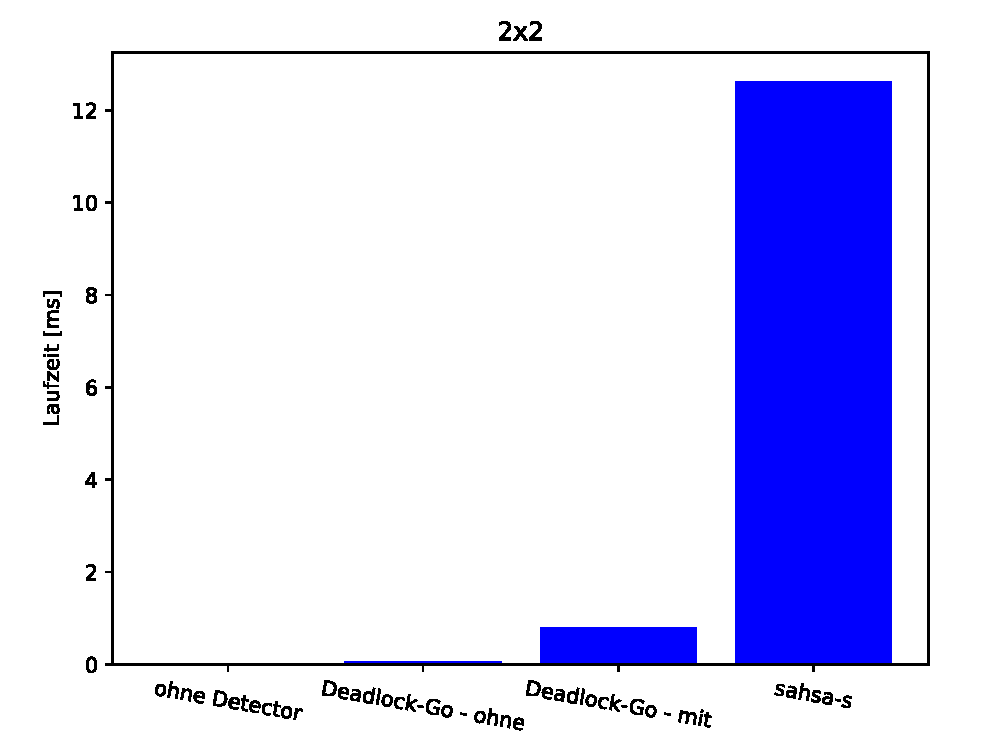
\includegraphics[width=.47\textwidth]{img/2x2_runtime.eps} & 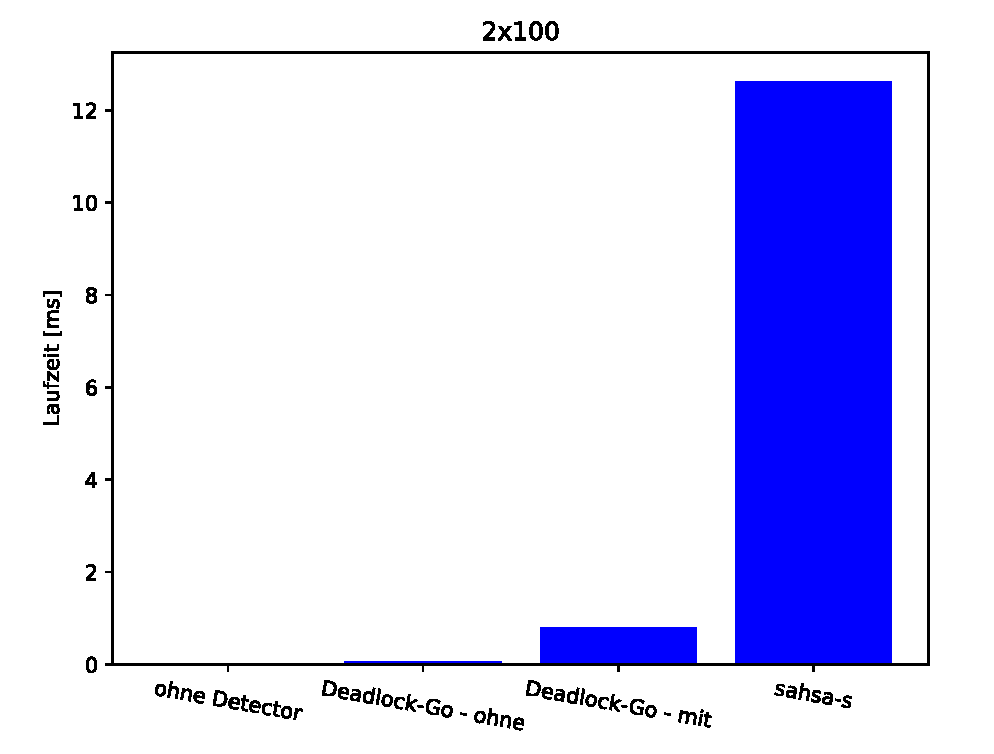
\includegraphics[width=.47\textwidth]{img/2x100_runtime.eps}\\
        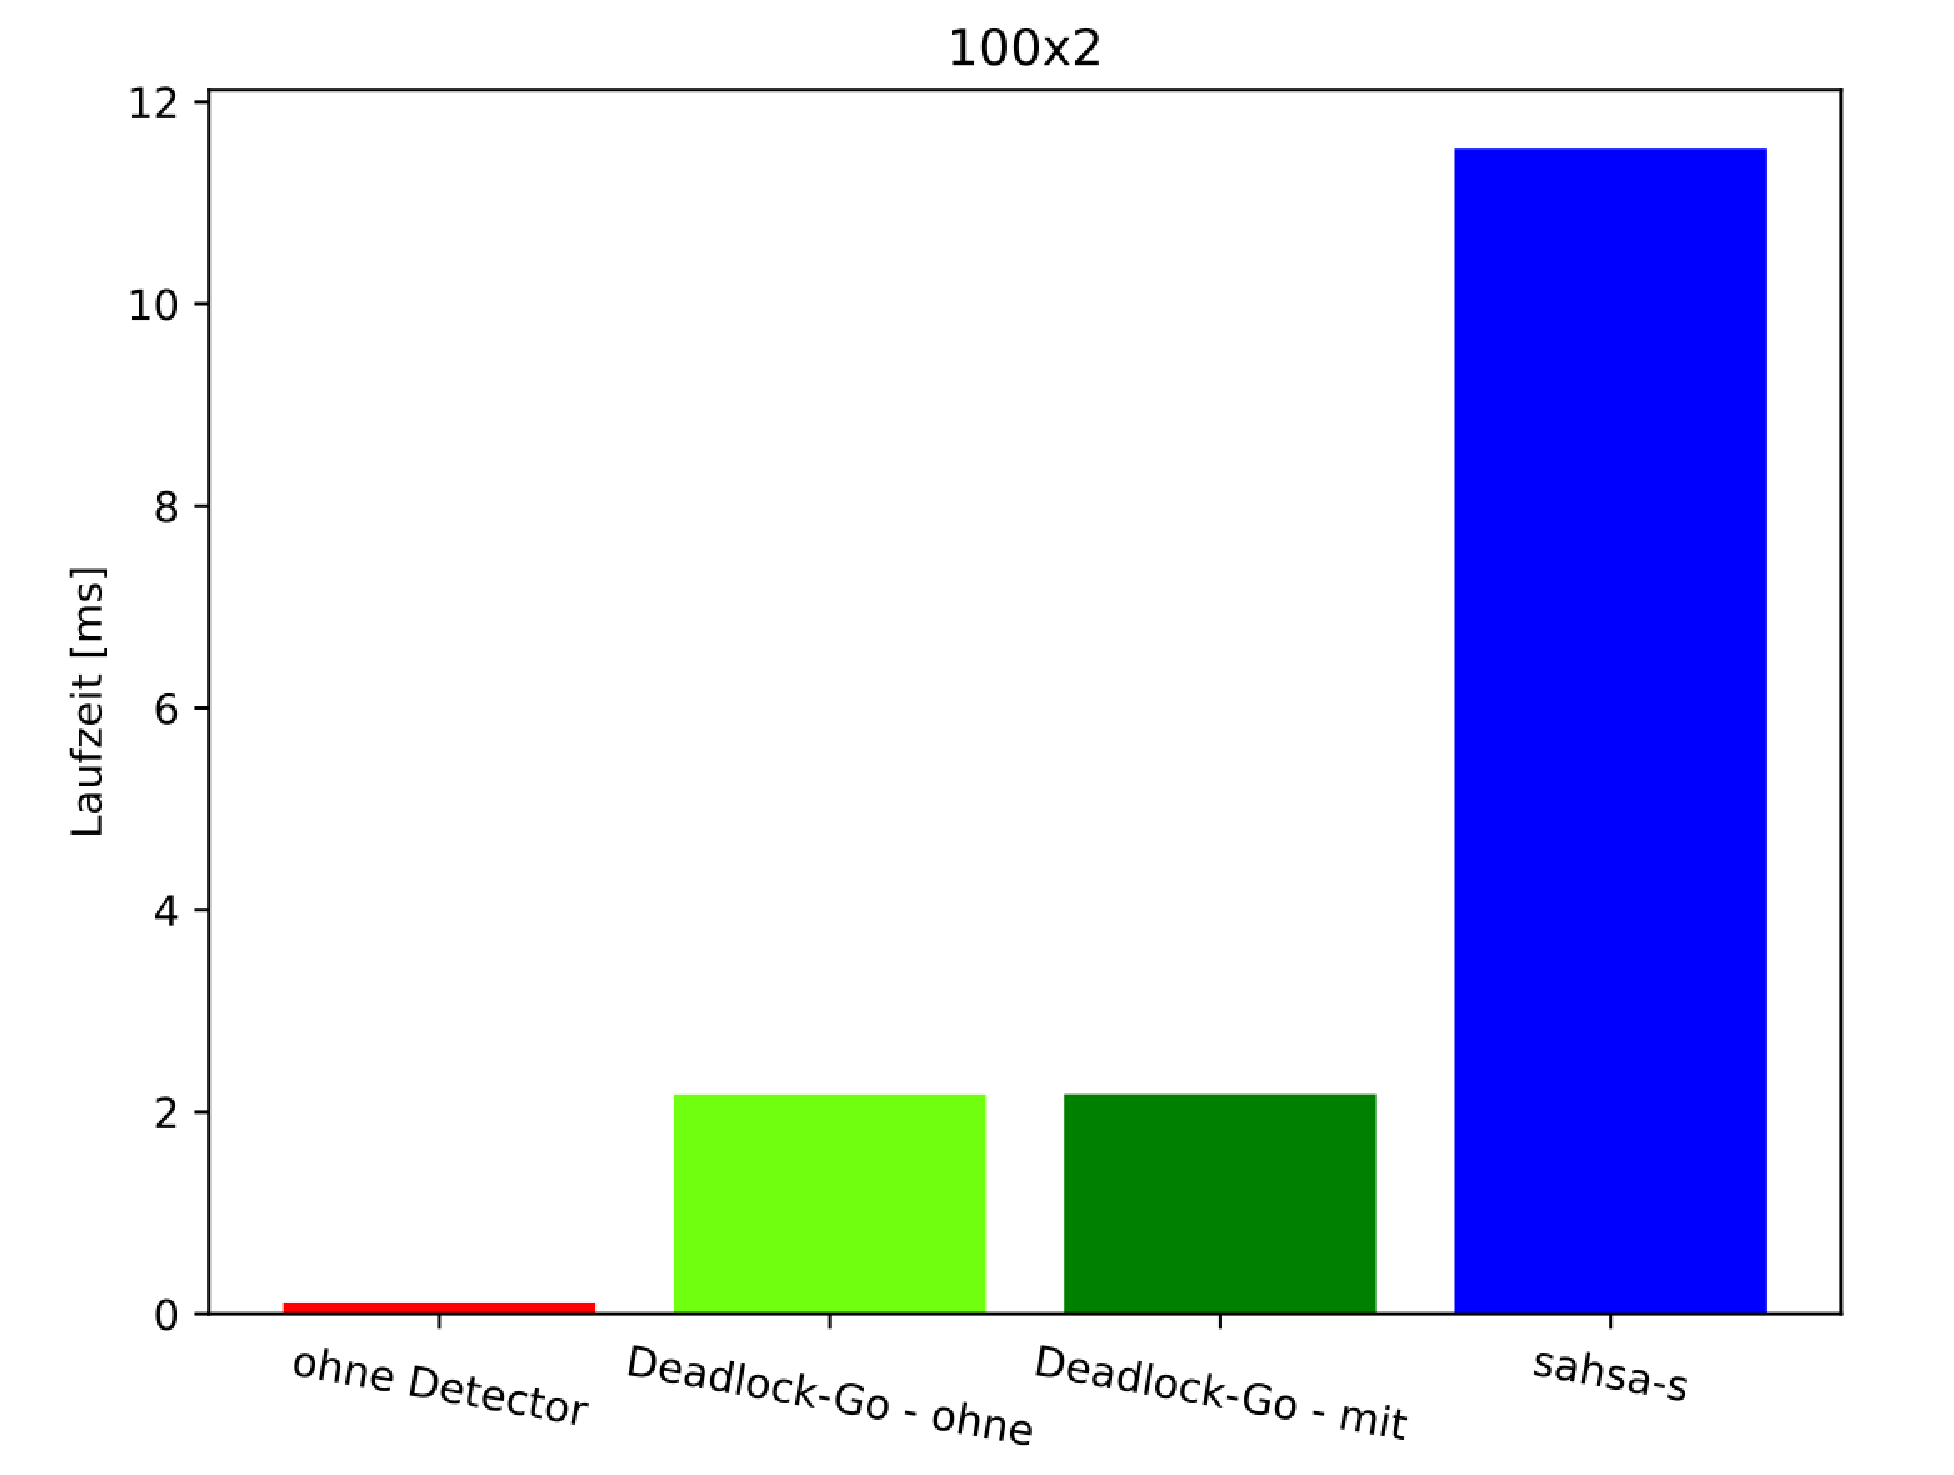
\includegraphics[width=.47\textwidth]{img/100x2_runtime.eps} & 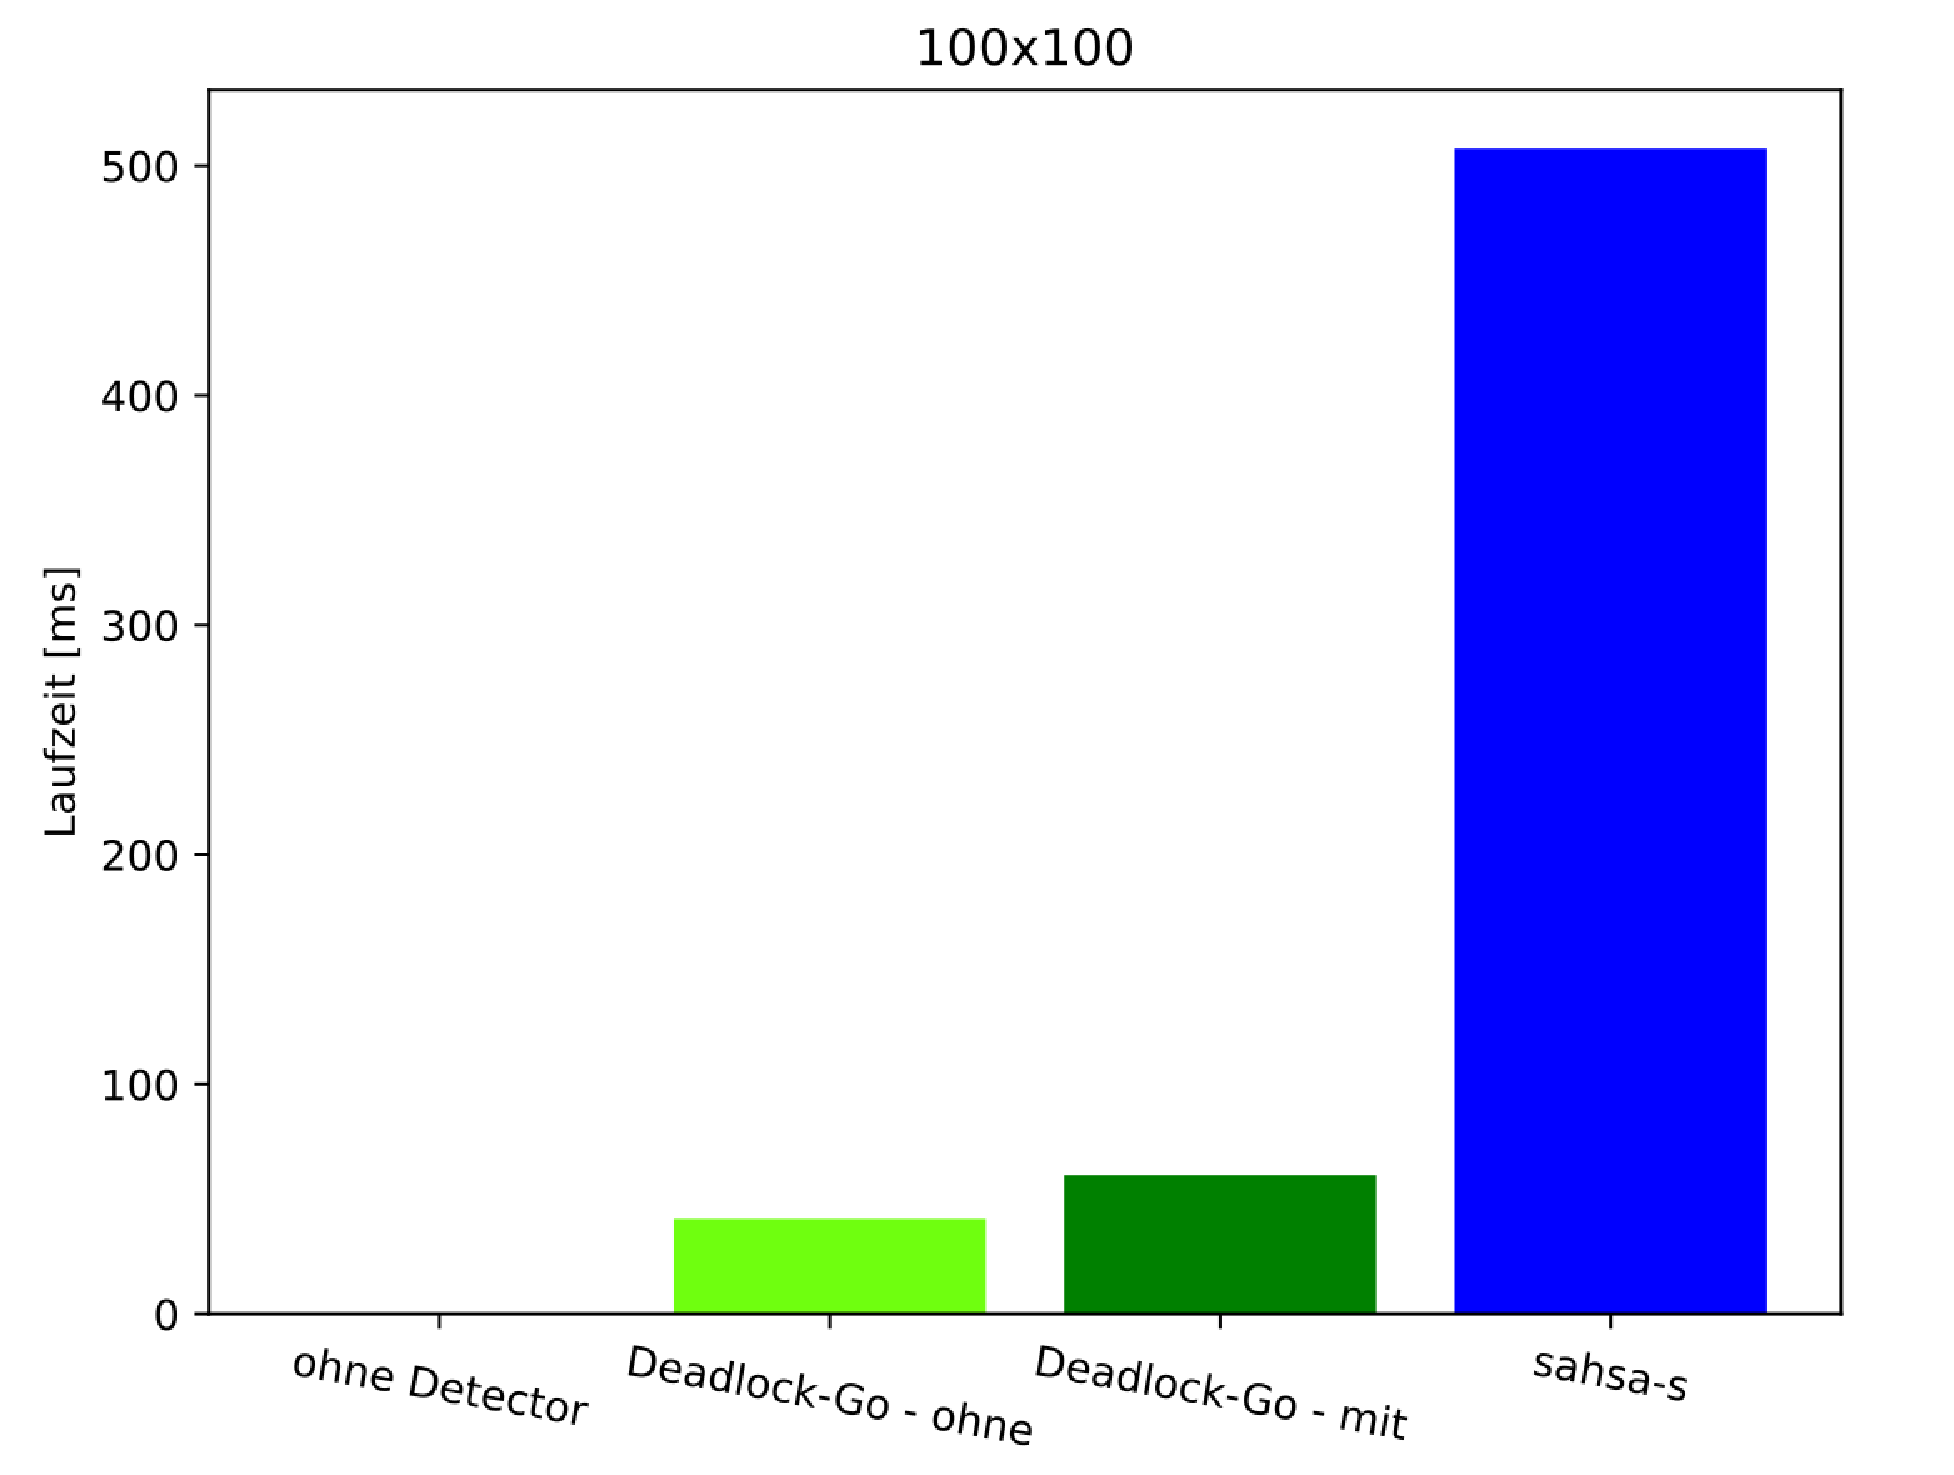
\includegraphics[width=.47\textwidth]{img/100x100_runtime.eps}\\
    \end{tabular}
    \caption{Laufzeiten dew eigentlichen Programms (ohne abschließende Detektion 
    in Deadlock-Go) der betrachteten Situationen ohne Detektor, mit Deadlock-Go und sasha-s. ``ohne'' und ``mit''
    für Deadlock-Go bedeutet dabei, dass der Detektor ohne bzw. mit periodischer 
    Detektion abgelaufen ist.}
\end{figure}
Es ist klar zu sehen, dass beide Detektoren die Laufzeit des eigentlichen 
Programms verlängern. Allerdings hat sasha-s dabei, sobald entweder die Anzahl der 
Locks oder Routinen größer wird, einen deutlich größeren 
Einfluss auf die Laufzeit. Dies liegt daran, dass Deadlock-Go während der 
Laufzeit des eigentlichen Programms nur Daten sammelt. Die 
periodische Detektion läuft dabei in einer eigenen Routine und hat daher 
nur einen geringen Einfluss auf die Laufzeit. Sasha-s hingegen sucht bereits 
während dem Ablauf des Programm nach potentiellen Deadlocks, und nutzt dabei 
die selben Routinen, mit denen das eigentliche Programm abläuft. Aus diesem Grund
hat sasha-s einen signifikant größeren Einfluss auf die Laufzeit des eigentlichen
Programms. \\\\
Betrachtet man die gesamte Laufzeit, also mit der abschließenden Detektion in 
Deadlock-Go, gibt sich allerdings folgendes Bild:

\begin{figure}[H]
\begin{tabular}{cc}
    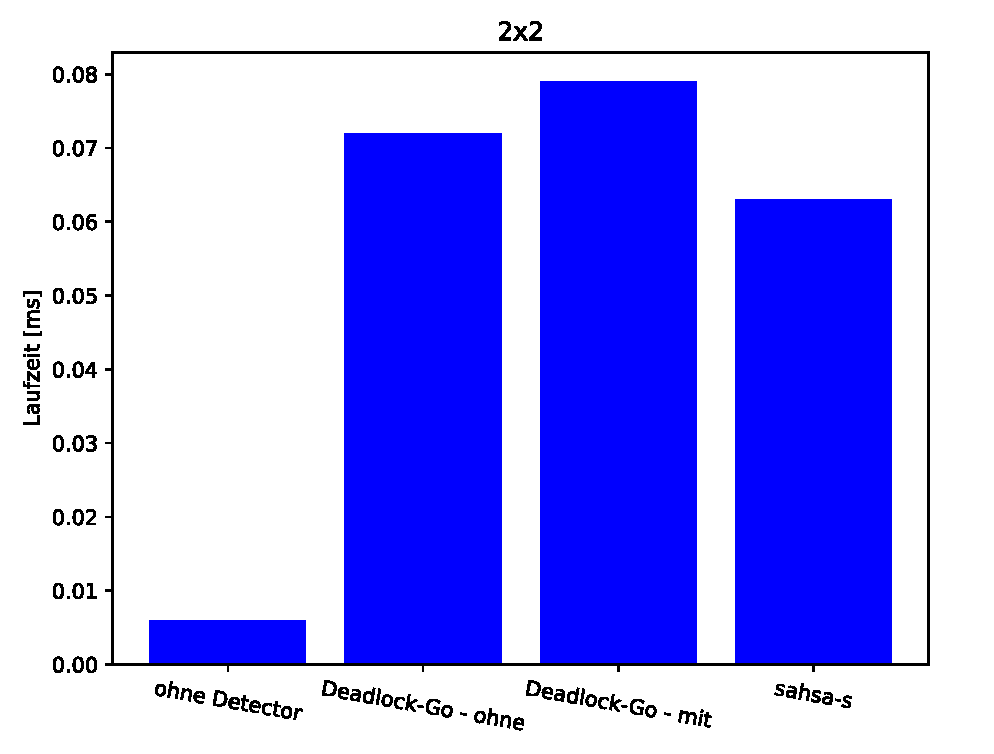
\includegraphics[width=.47\textwidth]{img/2x2.eps} & 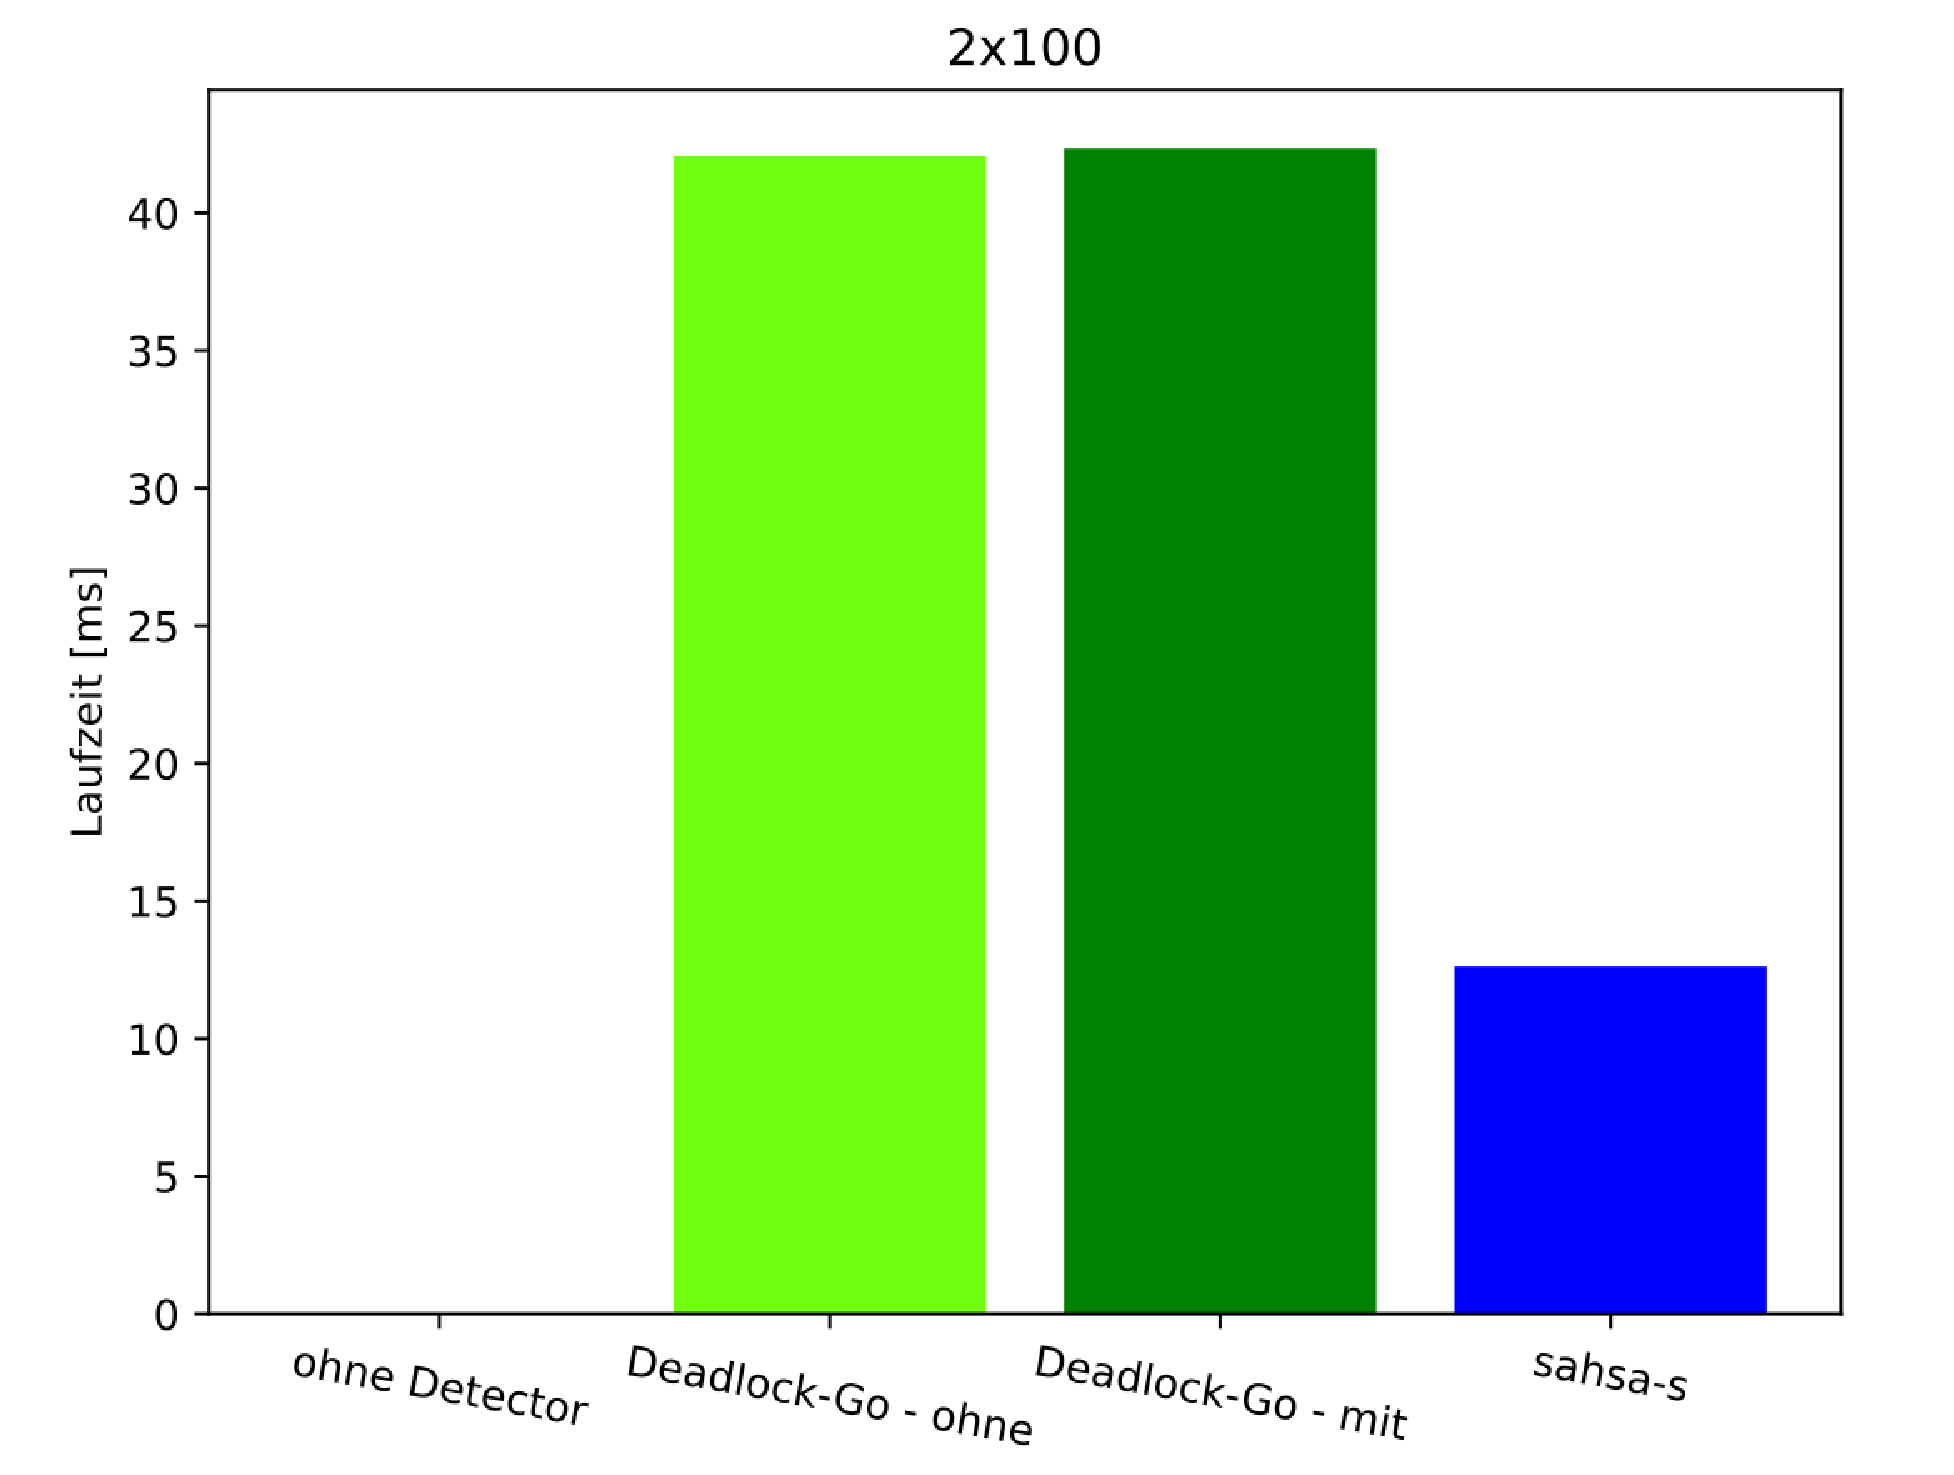
\includegraphics[width=.47\textwidth]{img/2x100.eps}\\
    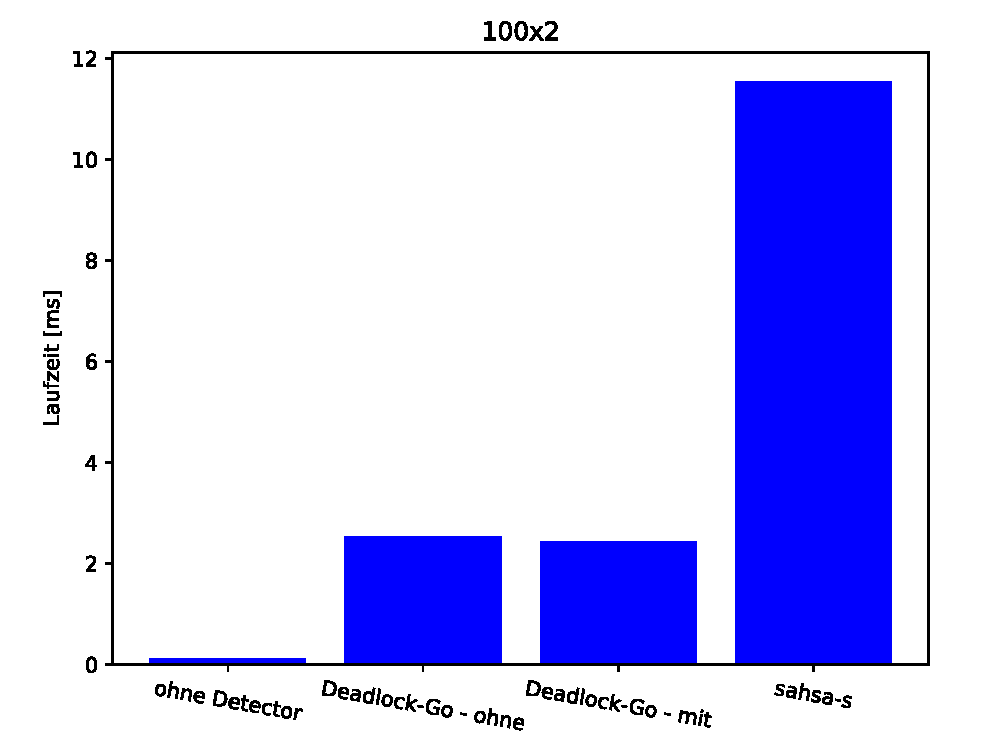
\includegraphics[width=.47\textwidth]{img/100x2.eps} & 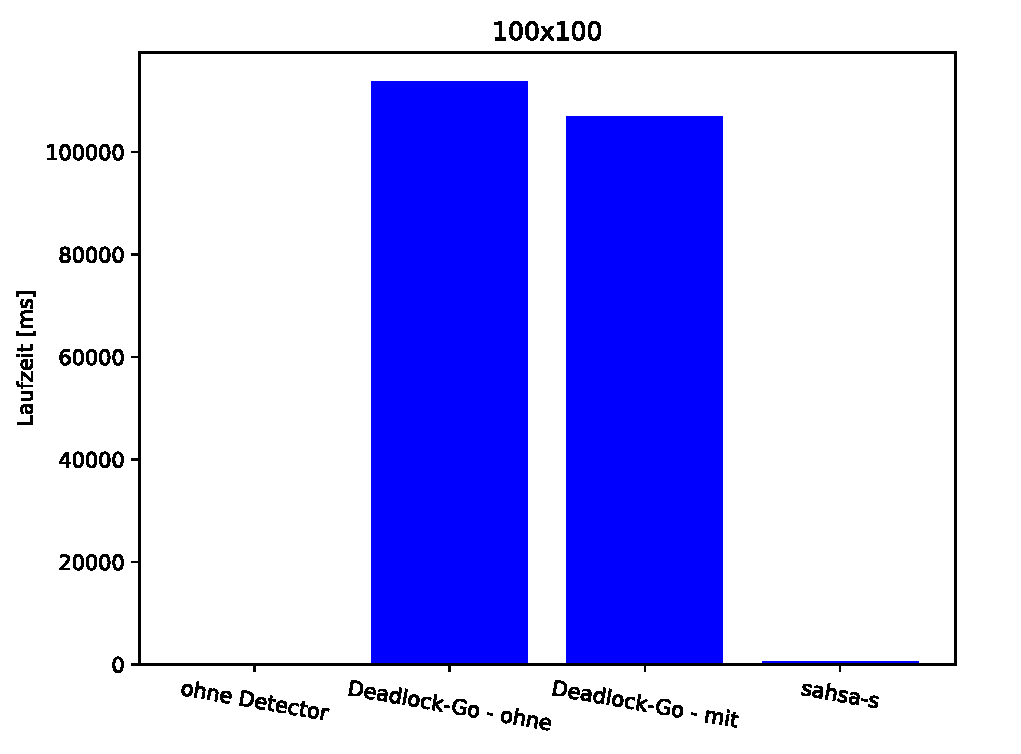
\includegraphics[width=.47\textwidth]{img/100x100.eps}\\
\end{tabular}
\caption{Gesammtlaufzeiten der betrachteten Situationen ohne Detektor, mit Deadlock-Go und sasha-s. 
    ``ohne'' und ``mit''
    für Deadlock-Go bedeutet dabei, dass der Detektor ohne bzw. mit periodischer 
    Detektion abgelaufen ist.}
\end{figure}
Bei dem Vergleich der beiden Detektoren bezüglich ihrer 
Laufzeit kommt es hier nun auf das betrachtete Programm an. Sind sowohl die Anzahl 
der Routinen als auch die Anzahl der Dependencies klein, ist der Unterschied
zwischen den beiden Detektoren relativ gering. Sasha-S hat einen klaren 
Vorteil, wenn es sich um ein Programm mit vielen Locks und damit vielen 
Dependencies handelt. Da sasha-s immer nur Pfade der Länge zwei in seinem 
Lock-Graphen betrachtet, 
währen Deadlock-Go alle möglichen Pfade in allen Kombinationen von Lock-Bäumen betrachtet, 
muss Deadlock-Go deutlich mehr Pfade analysieren, und hat daher eine signifikant
längere Laufzeit.
Deadlock-Go hat dafür einen Vorteil, wenn die Anzahl der 
Routinen groß, die Anzahl der Locks aber kein ist. Da die Lock-Bäume in Deadlock-go
in diesem Fall alle sehr klein sind, verliest sasha-s seine Vorteil, dass 
es nur Pfade der Länge 2 betrachtet. Allerdings überwiegt dieser wieder 
deutlich, wenn sowohl die Anzahl der Routinen als auch die Anzahl der Lock groß
ist.\\ \\
Beide Detektoren sind in der Lage, die Detektion zu deaktivieren, so dass sie dann nur noch einen
sehr geringe Verlängerung der Laufzeiten haben. Nachdem ein Programm zu Ende entwickelt
wurde, und alle potenziellen Deadlock beseitigt wurden, kann die Detektion somit deaktiviert
werden, um die schnelleren Laufzeiten zu erreichen, ohne dass der Detector aus dem Code entfernt
werden muss.